% 

\documentclass[10pt,a4]{article}

\usepackage{cogsci}
\usepackage{pslatex}
\usepackage{apacite}
\usepackage{graphicx}
\usepackage{csquotes}
\usepackage{tipa}


\title{Influences of Uncertainty Optimization on the Development of Language}
 
\author{{\large \bf Christopher Dilley} \\
	 christopher.dilley@student.uni-tuebingen.de \\\And
	{\large \bf Erik Schill} \\
	email@email.com \And
	{\large \bf Inna Pirina} \\
	email@email.com }


\begin{document}

\maketitle


\begin{abstract}
	
	This is where an abstract would go.
	
\end{abstract}


\section{Background}

In this paper, we aim to determine the linguistic relatedness of a number of languages in the same manner as described in \citeA{ellison2006measuring}, using an improved dataset.  

Kirby and Ellison describe a process whereby a language is quantified as a matrix comparing the probability of confusing one word for another for every word pair in the language, and these matrices are compared and clustered based on their relatedness.  By doing so, they achieved very encouraging results, automatically generating a phylogenic tree of languages that closely resembles the generally accepted phylogeny; the languages all fell neatly into their respective language subfamilies.

In employing a new set of data, we hoped to obtain equal or better results.  This new data set contains more data than that used by the authors in the paper, and uses each word's phonemic transcription rather than its orthography to calculate confusion probabilities.  We hypothesized that the language's phonemics would expose more meaningful relationships between words than orthography, as orthography can vary widely.  For example, the English words 'though' and 'toe' have significantly different orthography, while being pronounced very similarly (\textipa{[Do:]} and \textipa{[to:]}).

However, it is possible that this may give worse results as well.  Orthography may better represent the ancestry and relatedness of individual words, even when their phonetics converge.  The fact that 'though' and 'toe' are pronounced similarly may simply be due to random sound shifts causing phonetic convergence by chance, and this phonetic similarity may lead measures of word interrelatedness astray, negatively affecting intra-language comparisons. 

This study seeks to identify which of these hypotheses is more likely. \\

\textbf{- PHONETICS vs. PHONEMICS vs. PHONOLOGY... WHICH IS CORRECT USAGE HERE?} \\

\textbf{- THIS SECTION COULD PROBABLY BE EXPANDED}

\section{Implementation}

Our methodology follows much of the same procedures as Kirby and Ellison (2006).  We developed our own tools for generating the lexical metrics of all languages and for comparing them as well, while using an external tool to render the phylogenic trees from the resulting data.

As our input, we obtained data from the Indo-European Lexical Cognacy Database.  This data set spans 208 word meanings across 52 languages (not all languages had data for all word meanings), and includes phonemic transcriptions for all words.  We used these transcriptions instead of the word orthography for the inter-lexical comparisons, expecting to better detect similarity between words.

\subsection{Calculating Lexical Metrics}

(Talk about this process of comparing all words inside each language to generate the matrices)

Hey, look at the lexical metric in Figure~\ref{fig:french}.

\begin{figure}[ht]
\centering
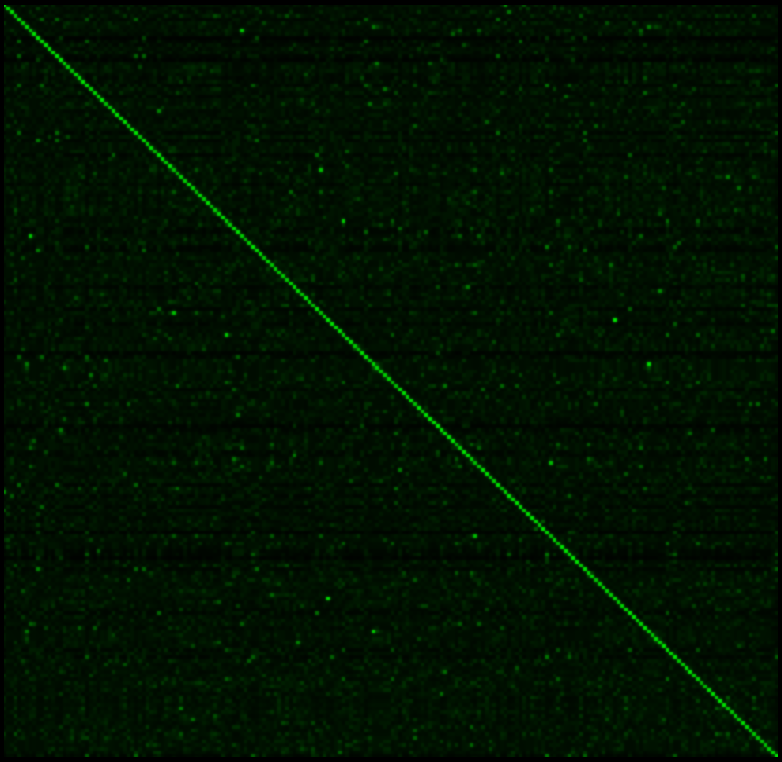
\includegraphics[width=0.8\linewidth]{french3}
\caption{A visualization of the lexical metric for French.}
\label{fig:french}
\end{figure}



\subsection{Calculating Language Distance}

(Talk about the process of comparing these matrices, and how we got around the various difficulties of languages not having certain words or having multiple words for a single meaning)

\subsection{Constructing Phylogenic Trees}

Once having constructed a matrix that represents the distance between all language pairs in the collection, these results need to be converted into an analyzable form.  Specifically, we want to visualize how close certain language pairs are related, and how they cluster together into larger groups.  From this, we hope to see some of the same taxonomic relations that are generally accepted as language families and subfamilies.

In order to accomplish this, we began by using the \textit{NEIGHBOR} program from the \textit{PHYLIP} package \cite{web:phylip}, as was done in the paper.  This program takes a matrix input, and constructs a tree that represents the relatedness of all of the languages based on their distance measurement.  This tree is output in a text form (in the standardized 'Newick' format) that describes the nodes on the tree and the distance to their child nodes.  Once having generated this, we used the Phylodendron tool from the University of Indiana to visualize this information as a proper tree \cite{web:phylodendron}.  

This process is repeated separately for each of the distance measurement matrices (the KL distance matrix and the Rao distance matrix).

\section{Results}

\section{Discussion and Conclusion}


\bibliographystyle{apacite}

\setlength{\bibleftmargin}{.125in}
\setlength{\bibindent}{-\bibleftmargin}

\bibliography{LVC}


\end{document}
